% !TEX encoding = UTF-8 Unicode
\documentclass[a4paper]{article}

% Dodato da se ne bi prikazivali podnaslovi u sadrzaju, a da ipak ostanu numerisani u okviru teksta
\setcounter{tocdepth}{1}    % levels under \subsection are not listed in the TOC


\usepackage{color}
\usepackage{url}
\usepackage[utf8]{inputenc} % make weird characters work
\usepackage{graphicx}


\usepackage[english,serbian]{babel}

\usepackage[unicode]{hyperref}
\hypersetup{colorlinks,citecolor=green,filecolor=green,linkcolor=blue,urlcolor=blue}

\usepackage{listings}

\newtheorem{primer}{Primer}[section]

\definecolor{mygreen}{rgb}{0,0.6,0}
\definecolor{mygray}{rgb}{0.7,0.7,0.7}
\definecolor{mymauve}{rgb}{0.58,0,0.82}

\lstset{ 
  backgroundcolor=\color{white},   % choose the background color; you must add \usepackage{color} or \usepackage{xcolor}; should come as last argument
  basicstyle=\scriptsize\ttfamily,        % the size of the fonts that are used for the code
  breakatwhitespace=false,         % sets if automatic breaks should only happen at whitespace
  breaklines=false,                 % sets automatic line breaking
  captionpos=b,                    % sets the caption-position to bottom
  commentstyle=\color{mygreen},    % comment style
  deletekeywords={...},            % if you want to delete keywords from the given language
  escapeinside={\%*}{*)},          % if you want to add LaTeX within your code
  extendedchars=true,              % lets you use non-ASCII characters; for 8-bits encodings only, does not work with UTF-8
%  firstnumber=1000,                % start line enumeration with line 1000
  frame=single,	                   % adds a frame around the code
  keepspaces=true,                 % keeps spaces in text, useful for keeping indentation of code (possibly needs columns=flexible)
  keywordstyle=\color{blue},       % keyword style
  language=Python,                 % the language of the code
  morekeywords={*,...},            % if you want to add more keywords to the set
%  numbers=left,                    % where to put the line-numbers; possible values are (none, left, right)
%  numbersep=0pt,                   % how far the line-numbers are from the code
%  numberstyle=\tiny\color{mygray}, % the style that is used for the line-numbers
  rulecolor=\color{black},         % if not set, the frame-color may be changed on line-breaks within not-black text (e.g. comments (green here))
  showspaces=false,                % show spaces everywhere adding particular underscores; it overrides 'showstringspaces'
  showstringspaces=false,          % underline spaces within strings only
  showtabs=false,                  % show tabs within strings adding particular underscores
%  stepnumber=2,                    % the step between two line-numbers. If it's 1, each line will be numbered
  stringstyle=\color{mymauve},     % string literal style
  tabsize=2,	                   % sets default tabsize to 2 spaces
  title=\lstname                   % show the filename of files included with \lstinputlisting; also try caption instead of title
}

\renewcommand{\lstlistingname}{Kod}% Listing -> Algorithm
\renewcommand{\lstlistlistingname}{List of \lstlistingname s}%

\begin{document}

\title{Prepoznavanje saobraćajnih znakova pomoću konvolutivnih neuronskih mreža\\ \small{Seminarski rad u okviru kursa\\Računarska inteligencija\\ Matematički fakultet}}

\author{Jana Jovičić 215/2015, Jovana Pejkić 435/2016 \\ jana.jovicic755@gmail.com, jov4ana@gmail.com}

\date{16.~maj 2019.}

\maketitle

\abstract{

}

\newpage

\tableofcontents

\newpage

\section{Uvod}
\label{sec:uvod}

Klasifikacija je vrsta problema nadgledanog učenja <FUSNOTA> koja podrazumeva predvidjanje kategoricke ciljne promenljive. Kategorickim se smatraju promenljive koje uzimaju konacan broj vrednosti (medju kojima nema uredjenja). Na primer, prepoznavanje da li je dobijen e-mail spam, reklama ili obicna poruka je problem klasifikacije.

Prepoznavanje i klasifikacija slika je polje u oblasti mašinskog učenja koje se veoma brzo razvija. Na primer, klasifikatori slika (mada se već koriste) će se sve više koristiti za: zamenu lozinke prepoznavanjem lica, prepoznavanje otisaka prstiju, analizu krvnih slika, identifikaciju geografskih karakteristika iz satelitskih snimaka, analizu aero i satelitskih snimaka, detekciju urbanih područja, detekciju puteva, autonomnu vožnju i otkrivanje prepreka itd.

Postoje mnogi algoritmi koji se koriste za klasifikaciju slika (npr. SVM), a jedan od najboljih je CNN - konvolutivne neuronske mreže. CNN se može zamisliti kao automatski ‚‚ekstraktor’’ karakteristika slike. On efikasno koristi informacije o susednim pikselima da bi efektivno konvolucijom smanjio sliku, a zatim da bi predvideo kategoriju kojoj slika pripada, koristi sloj za predviđanje. Iako su konvolutivne neuronske mreže projektovane tako da prednost postižu u radu sa 2D strukturama, kao što su slike ili ulazi poput govornog signala (eng. speech signal), najnovije studije pokazuju da postižu značajne rezultate i sa 3D strukturama.

Svrha ovog rada je da prikaže osnovne osobine konvolutivnih neuronskih mreža i da pokaže na koji način se one mogu implementirati tako da korektno identifikuju saobraćajne znakove iz baze podataka sa kineskim saobraćajnim znacima. U radu je opisano nekoliko modela mreža i upoređeni su njihovi ostvareni rezultati.


%Svrha implementacije konvolutivne neuronske mreže o kojoj ovaj rad govori jeste da korektno identifikuje saobraćajne znakove iz baze podataka sa kineskim saobraćajnim znacima. U radu je opisana implementacija ove mreže i diskutovano je o ostvarenim rezultatima.

\newpage

\section{Neuronske mreže}
\label{sec:cnn}

%U masinskom ucenju, neuronske mreze (eng. neural networks) vaze za jednu od najprimenjenijih metoda.
Neuronske mreže predstavljaju skup statističkih modela učenja inspirisane biološkim neuronima, za rešavanje klasifikacionih\footnote{Klasifikacioni problem - ako je izlazna promenljiva kategorickog tipa, npr. ,,zdrav" i ,,bolestan".} i regresionih problema\footnote{Regresioni problem - ako je izlazna promenjiva neprekidnog tipa, npr. ,,plata" ili ,,tezina".}. Njihove primene su mnogobrojne, a neke od njih su: kategorijzacija teksta,
%prepoznavanje rukom pisanih tekstova, medicinska dijagnostika, prepoznavanje objekata na slikama, robotika i automatsko upravljanje,
 raspoznavanje i sinteza govora, autonomna voznja, igranje video igara, masinsko prevodenje prirodnih jezika i slicno. Kljucna prednost neuronskih mreza je da same mogu da konstruisu nove atribute nad sirovom reprezentacijom podataka\footnote{Iako se nekad mogu pretpostaviti koji su atributi najinformativniji za predvidanje ciljne promenljive, izbori tih atributa su neretko losiji od onoga sto bi algoritam ucenja mogao da detektuje u sirovoj informaciji.} i odlicno baratanje sa velikim kolicinama podataka.
 %Za male kolicine podataka neuronske mreze nisu pogodne jer lako vode preprilagodavanju, stoga obim podataka igra bitnu ulogu.


\subsection{Arhitektura}

Osnovnu jedinicu gradje neuronske mreze predstavljaju neuroni, koji su medjusobno povezani vezama sa tezinama koje se podesavaju tokom ucenja mreze. Povezani neuroni prosledjuju signale jedni drugima, a organizovani su u slojeve. Najjednostavniji oblik neuronske mreze je perceptron, koji sadrzi samo jedan ulazni i jedan izlazni sloj. Medjutim, kako on sluzi samo za ucenje linearnih modela, a u praksi se javlja potreba da i slozeniji modeli mogu da se nauce, osim perceptrona, koriste se viseslojne neuronske mreze. Viseslojna neuronska mreza osim ulaznog i izlaznog sloja, ima jedan ili vise skrivenih slojeva (slika \ref{fig:neural_network_layers}).
%Broj skrivenih slojeva je proizvoljan, dok sama struktura skrivenog sloja utice na performanse mreze.
Kako se neuronske mreze uglavnom koriste za klasifikaciju uzorka u razlicite kategorije, ulazni sloj se sastoji od onoliko neurona kolika je dimenzionalnost ulaznog prostora, a broj neurona na izlazu jednak je broju klasa. Samo ucenje neuronske mreze je zapravo podesavanje tezina sve dok se ne dobije zadovoljavajuca aproksimacija izmedju ulaznih i izlaznih velicina.

\begin{figure}[h!]
\begin{center}
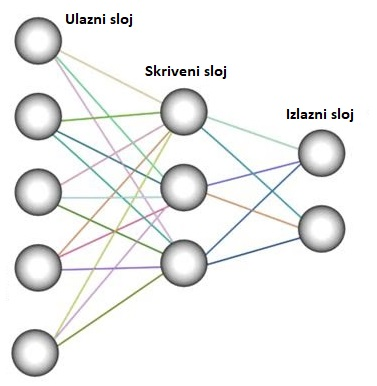
\includegraphics[scale=1]{neural_network_layers.jpeg}
\end{center}
\caption{Višeslojna neuronska mreža sa jednim skrivenim slojem}
\label{fig:neural_network_layers}
\end{figure}


\subsection{Razlog uvodjenja CNN}
Jednostavni zadaci prepoznavanja mogu se dosta dobro resiti skupovima podataka malih velicina, na primer desetine hiljada slika. Medjutim, objekti u realisticnim postavkama pokazuju znacajnu varijabilnost, stoga, da bi bilo moguce nauciti prepoznati ih, potrebno je koristiti mnogo vece skupove za treniranje. Da bismo naucili o hiljadama objekata iz miliona slika, potreban nam je model sa velikim kapacitetom ucenja. Konvolutivne neuronske mreze (CNN), koje ce biti detaljno obradjene u ostatku rada, cine jednu takvu klasu modela. ne daju jake i uglavnom ispravne pretpostavke o prirodi slika, a njihov kapacitet se moze kontrolisati variranjem njihove dubine i sirine. Tako, u poredjenju sa standardnim (feedforward) neuronskim mrezama sa slojevima slicnih velicina, CNN imaju mnogo manje veza i parametara, tako da ih je lakse trenirati, dok je njihov teoretski najbolji ucinak verovatno samo nesto losiji.


\section{Konvolutivne neuronske mreže}	
\label{sec:podnaslov3}

%\cite{ime_knjige}.

Konvolutivne neuronske mreze (eng. Convolutional neural network, CNN) predstavljaju podklasu neuronskih mreza koja ima najmanje jedan konvolutivni sloj (a moze ih imati i vise). Ova vrsta neuronskih mreza je inspirisana vizuelnim korteksom. Svaki put kada nešto vidimo, aktivira se niz slojeva neurona, i svaki sloj otkriva skup karakteristika kao što su linije, ivice itd. Visi nivoi slojeva otkritivaju složenije karakteristike kako bi prepoznali ono što smo videli. Konvolutivne mreze rade po istom principu i prakticno su uvek duboke neuronske mreze, upravo zbog toga sto je potrebno od sitnijih detalja, poput uspravnih, kosih i horizontalnih linija, koji obicno bivaju detektovani u nizim slojevima mreze, konstruisati slozenije oblike poput delova lica. Konvolutivne neuronske mreze se koriste u obradi signala (slike, zvuka), ali i teksta. U odnosu na ostale vrste neuronskih mreza, isticu se u prikupljanju lokalnih informacija (na primer o susednim pikselima na slici ili ,,okruzujucim" (eng. surrounding) recima u tekstu) i smanjenju slozenosti modela (brze treniranje, potrebno je manje izoraka, manja sansa da dodje do preprilagodjavanja (eng. overfitting)). Konvulativne neuronske mreze se zasnivaju na sposobnosti mreza da iz sirovog signala konstruisu atribute. Nazivaju se konvolutivnim zato sto uce \textbf{filtere} (pojam objasnjen u tabeli \ref{tabela_parametri}), cijom konvolutivnom primenom detektuju odredjena svojstva signala.

Postoji nekoliko arhitektura u polju konvolutivnih neuronskih mreža, koje se razlikuju po tipu, broju i rasporedu slojeva. Dve najpoznatije su:

\begin{itemize}

\item LeNet-5 - ovu arhitekturu je napravio Yann LeCunn krajem 20. veka, a koristila se za citanje zip kodova, cifara itd. LeNet-5 arhitektura se sastoji iz dva skupa konvolutivnih slojeva (eng. convolutional layers) i slojeva agregacije (eng. average pooling layers), koji su praćeni poravnavajućim konvolutivnim slojem (eng. flattening convolutional layer), a onda slede dva potpuno-povezana sloja (eng. two fully-connected layers) i konačno softmax klasifikator (eng. softmax classifier).

\item AlexNet je jedna od prvih dubokih neuronskih mreža. Sastoji se iz pet konvolutivnih slojeva praćena sa tri potpuno povezana sloja.
Ovu mrežu je napravio Alex Krizhevsky, koji je koristio prečišćenu linearnu jedinicu (eng. Rectified Linear Unit, ReLu)\footnote{ReLu funkcija se definiše kao: f(x) = max(0,x). Prednost ReLu nad sigmnoidnom funkcijom je što treniranje obavlja mnogo brže.} za ne-linearni deo umesto Tanh ili Sigmoid funkcije, koje su bile standardne za tradicionalne neuronske mreže.

%\item VGG16 predstavlja unapređenje arhitekture AlexNet. U njoj su veliki filteri (jezgra) zamenjeni sa više malih 3x3 filtera jedan za drugim\footnote{Više manjih filtera se pokazuje boljim nego jedan veliki filter (jezgro), zato što više ne-linearnih slojeva povećavaju dubinu mreže što im omogućava da uče kompleksnije karakteristike (i to po manjoj ceni).}.

%\item GoogLeNet ima čak 22 sloja. Brža je i manja od Alexnet i mnogo preciznija. Ideja ove mreže jeste da se napravi model koji će moći da se koristi i na pametnom telefonu (eng. smart-phone).


\end{itemize}


% U narednoj tabeli su opisani neki od bitnijih parametara koje treba podesiti pri ucenju mreze.

\subsection{Parametri}

U ovoj sekciji je dat tabelarni prikaz parametara koji su najznacajniji za implementaciju konvolutivne mreze. U tabeli \ref{tabela_parametri} je dat samo kratak opis svakog od njih radi boljeg razumevanja teksta koji sledi. Ipak, u nastavku je svaki detaljnije opisan.

\begin{table}[h!]
\begin{center}
\caption{Primer tabele}
\begin{tabular}{|l|p{60mm}|}
\hline
Filter (jezgro, kernel) &
- matrica sa tezinama za konvoluciju ulaza \newline
- daje meru koliko deo ulaza liči na karakteristiku \newline
- tezine u matricama filtera su izvedene za vreme treniranja podataka
\\
\hline
Padding &
- koristi se za dodavanje kolona i redova nula da bi se odrzala konstantna velicina matrice (mape) nakon konvolucije \newline
- ovaj parametar moze da unapredi performanse tako sto zadrzava informacije u okvirima
\\
\hline 
Stride &
- broj piksela koji želite preskočiti, dok prelazite ulaz vodoravno i uspravno tokom konvolucije, nakon mnozenja svakog elementa iz ulazne matrice težina s onima u filtru
\\
\hline 
Number of Channels &
- It is the equal to the number of color channels for the input but in later stages is equal to the number of filters we use for the convolution operation. \newline
- The more the number of channels, more the number of filters used, more are the features learnt, and more is the chances to over-fit and vice-versa.
\\
\hline 
Pooling-layer Parameters &
- ima iste parametre kao i konvolutivni sloj \newline
- uglavnom se koristi Max-Pooling opcija \newline
- The objective is to down-sample an input representation (image, hidden-layer output matrix, etc.), reducing its dimensionality by keeping the max value(activated features) in the sub-regions binned.
\\
\hline 
\end{tabular}
\label{tabela_parametri}
\end{center}
\end{table}


\subsection{Konvolucija slika preko CNN}

%\ref{sec:ime_necega}.

Da bi izvrsile klasifikaciju slika, konvolutivne mreze (preciznije, konvolutivni sloj, detaljnije u poglavlju ?????) obavljaju neku vrstu pretrage. Ovo se moze zamisliti kao mali pokretni (ili klizni) prozor (prikazano na slici \ref{fig:filter_movement01}) koji klizi s leva na desno preko vece slike, i nastavlja s leve strane kada dodje do kraja jednog prelaza (kao kod pisace masine). Taj pokretni (klizni) prozor - koji ustvari predstavlja filter, moze da prepozna samo jednu stvar, recimo kratku vertikalnu liniju (tri tamna piksela naslagana jedan na drugi). Slicno, neki drugi filter moze da sluzi za prepoznavanje horizontalnih linija, i on se takodje pomera preko piksela slike, trazeci podudaranja. Rezultat koji se postize filterima koji prepoznaju vertikalne i horizontalne linijije prikazan je na slici \ref{fig:edges}.

% TODO: Slike se ne prikazuju u .pdf fajlu tamo gde su pozicionirane u .tex fajlu, iako je navedeno [h!]

\begin{figure}[h!]
\begin{center}
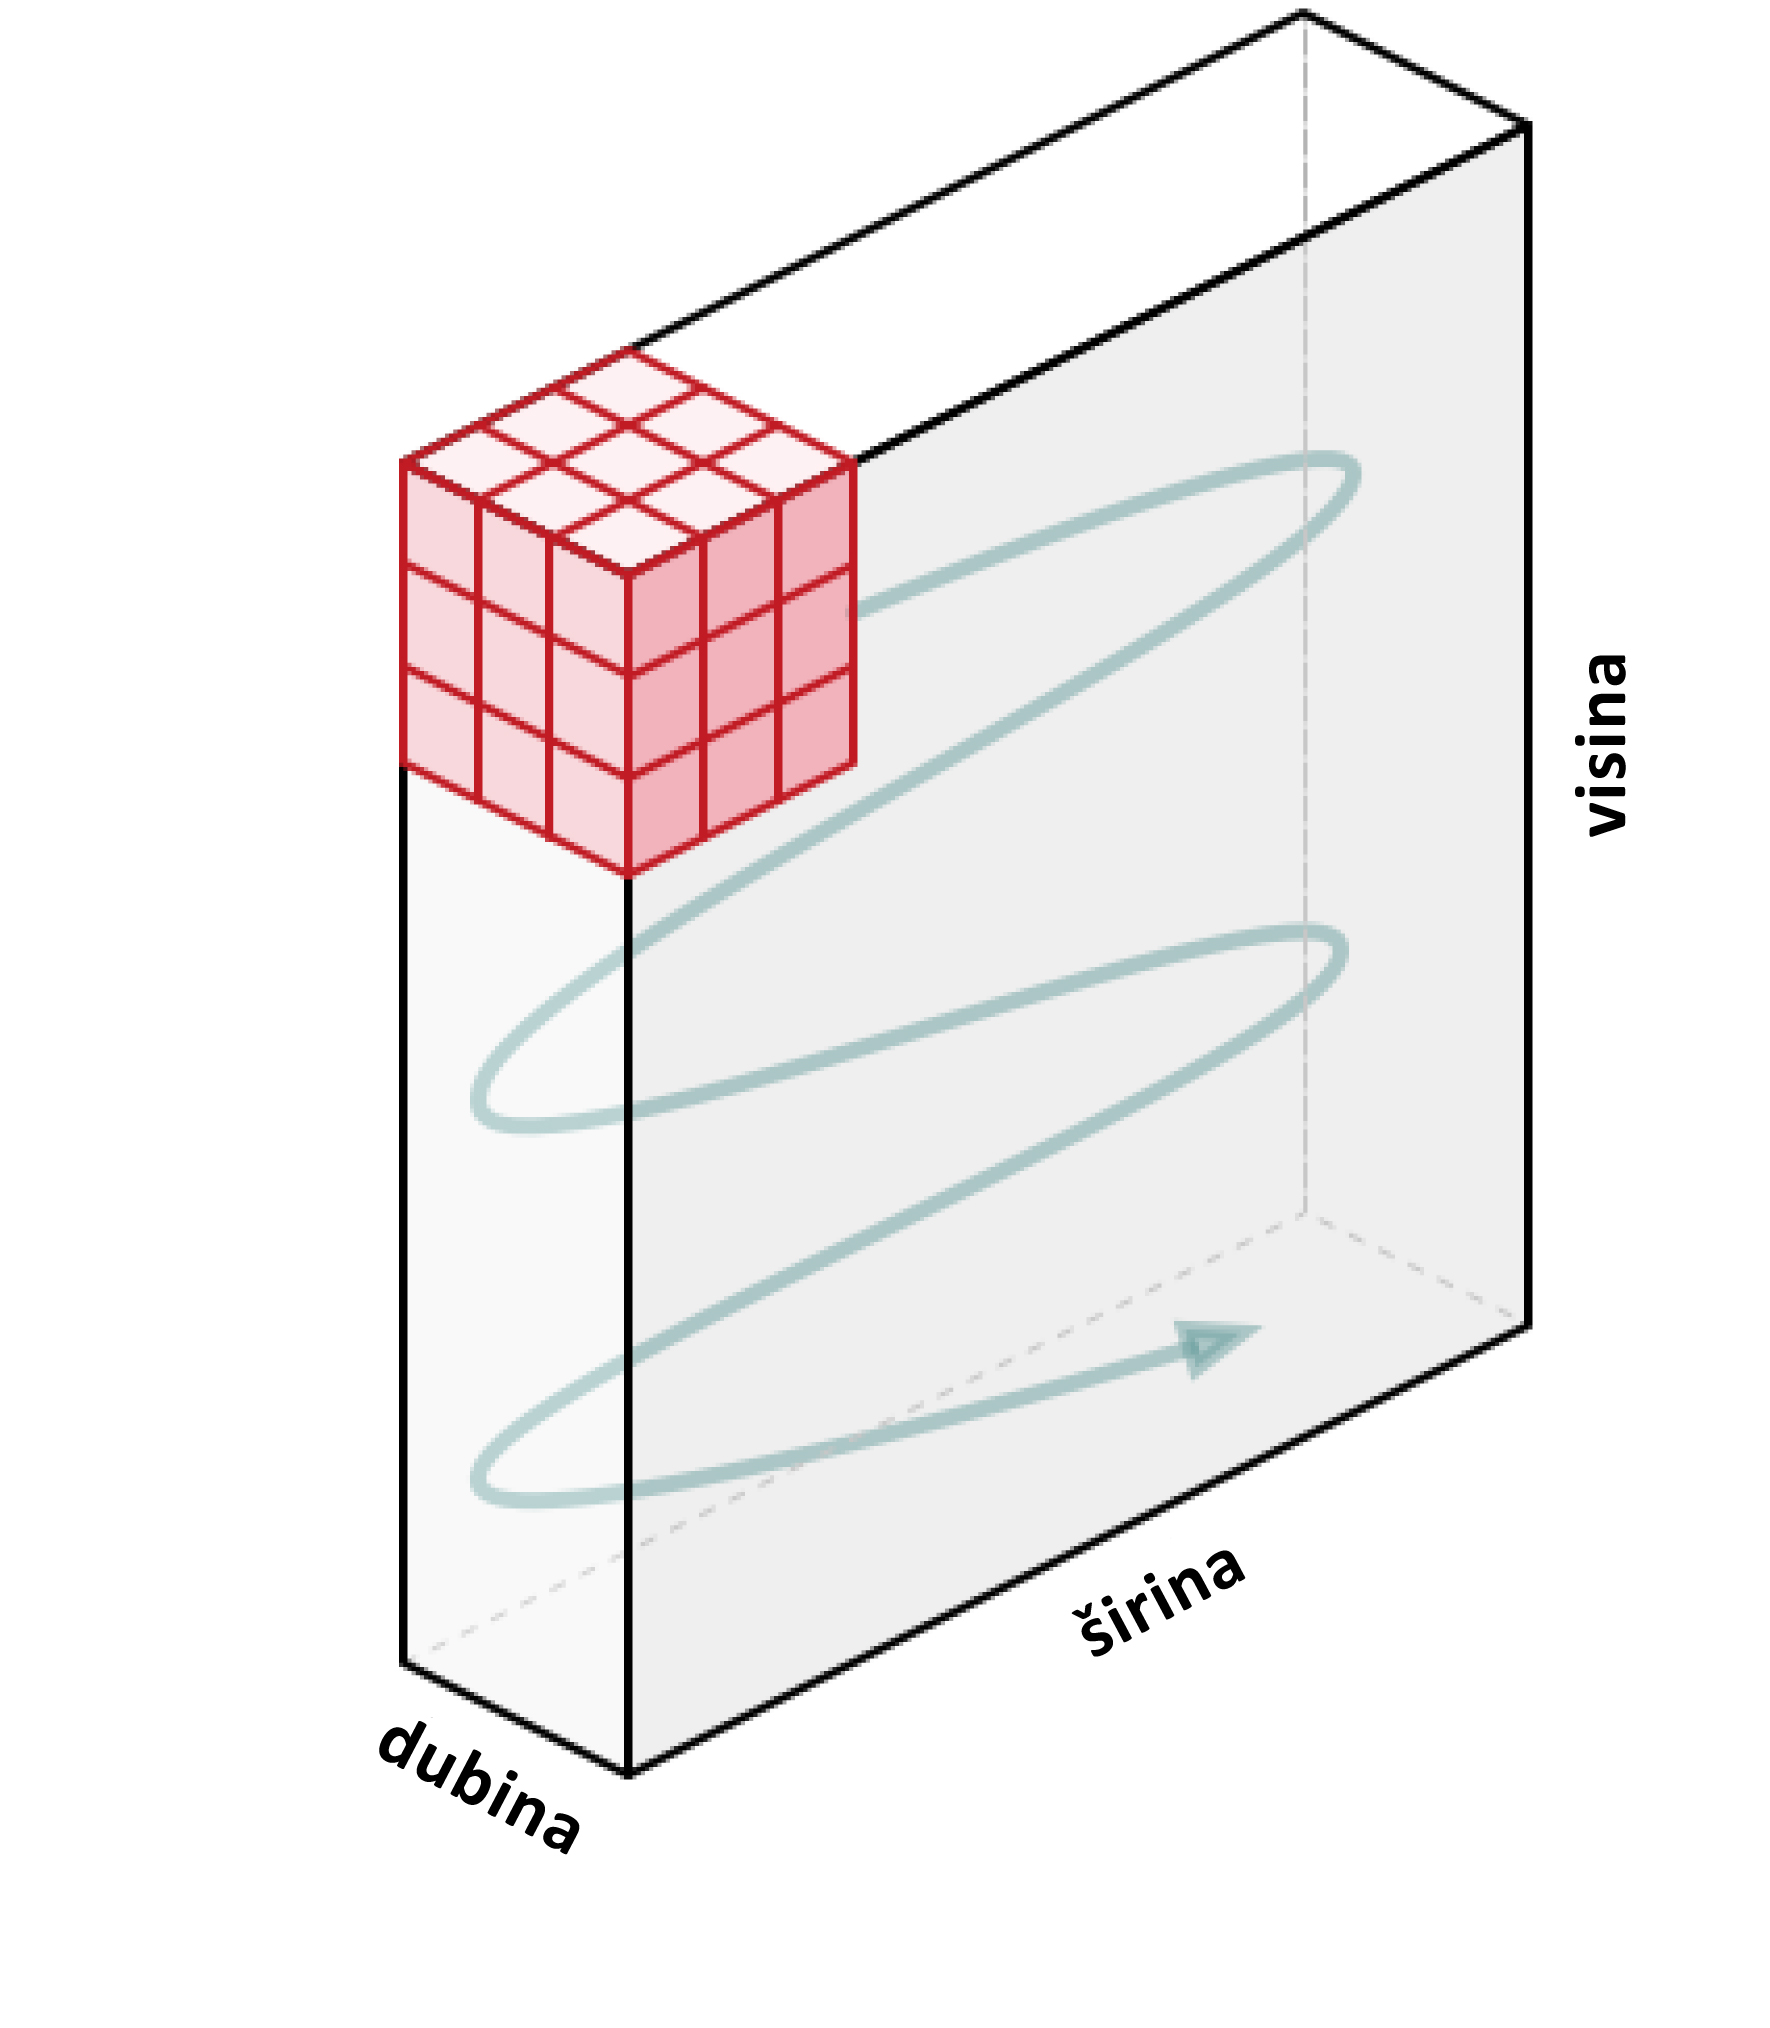
\includegraphics[scale=0.4]{filter_movement01.jpg}
\end{center}
\caption{Kretanje filtera}
\label{fig:filter_movement01}
\end{figure}


\begin{figure}[h!]
\begin{center}
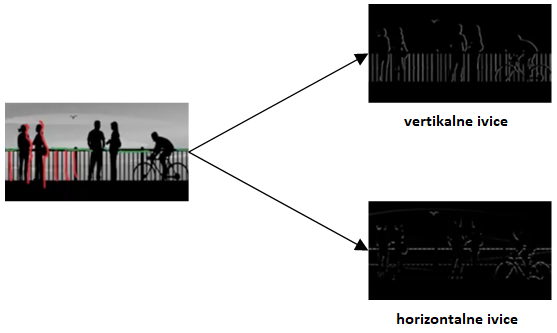
\includegraphics[scale=1]{edges.png}
\end{center}
\caption{Detektovanje ivica}
\label{fig:edges}
\end{figure}

Svaki put kada dodje do poklapanja (filtera sa ulazom), ono se mapira u prostor sa karakteristikama - koji se zove \textbf{mapa karakteristika} (eng. feature maps), koji je specifican za taj vizuelni element. U tom prostoru (tj. mapi) se cuva (odnosno belezi) lokacija svakog poklapanja sa vertikalnom linijom. Konvolutivna mreza pokrece mnogo pretraga nad jednom istom slikom. Na pocetnom sloju mreze koriste se filteri koji prepoznaju horizontalnu liniju, vertikalnu liniju i dijagonalnu liniju, da bi kreirali mapu ivica slike. U narednim koracima (odnosno slojevima) posmatraju se kombinacije ovih ivica i tako prepoznaju slozeniji oblici. Ovo je demonstrirano na slici \ref{fig:learning}.

\begin{figure}[h!]
\begin{center}
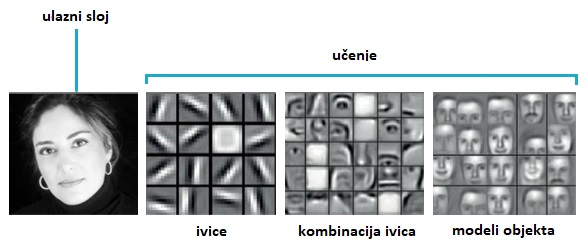
\includegraphics[scale=0.9]{learning.jpg}
\end{center}
\caption{Učenje mreže}
\label{fig:learning}
\end{figure}


\subsection{Unutrasnja struktura CNN}

Unutrasnja struktura konvolutivne mreže se sastoji od nekoliko naizmeničnih konvolutivnih slojeva (eng. convolution layer) i slojeva agregacije (eng. pooling layer), pri cemu je dozvoljeno pojavljivanje iste vrste sloja vise puta (prikazano na slici \ref{fig:cnn_layers}). U dosad opisanoj strukturi neurona (neuronskih mreza) izlaz iz svakog od njih je bio skalarna veličina. Izlazi konvolutivnog sloja su dvodimenzionalni i nazivaju se mapama karakteristika (eng. feature maps). Oni se transformisu nelinearnom aktivacionom funkcijom. U konvolutivnim mrežama kao aktivacione funkcije najčešće koriste ReLU (na izlazu iz konvolutivnog sloja) i Softmax (na izlazu iz poslednjeg, potpuno povezanog, sloja mreže). O njima će biti više reči u narednim poglavljima.

% TODO: Reci nesto o ostalim slojevima: Pooling layer i FC!

% TODO: Proveriti jos jednom za: (na primer tanh), koja ce prevesti ulazne vrednosti u opseg izmedju -1 i 1 (pretposlednja recenica)!


\begin{figure}[h!]
\begin{center}
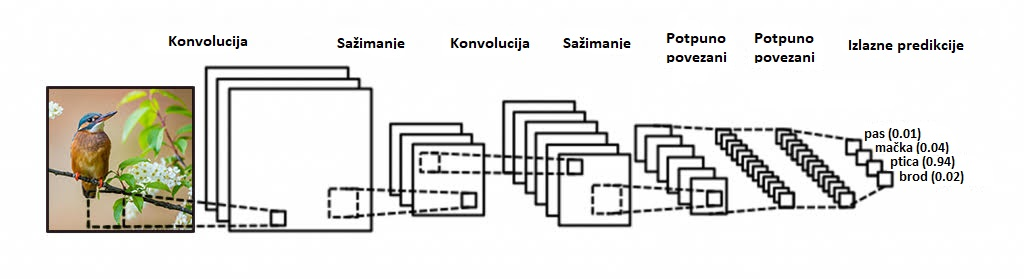
\includegraphics[scale=0.62]{cnn_layers.jpg}
\end{center}
\caption{Arhitektura konvolutivne neuronske mreže}
\label{fig:cnn_layers}
\end{figure}


\subsection{Konvolucija}
\label{konvolucija}

Konvolutivni sloj je glavni deo konvolutivne neuronske mreze koji radi najvise izracunavanja u mrezi. Njegova uloga je konstrukcija novih atributa. To je prvi sloj koji ekstraktuje karakteristike iz ulazne slike. Konvolucija je matematicka operacija koja uzima dva ulaza - dve matrice f i g, dimenzija m x n i p x q, a definisana je na sledeci nacin:
$$(f * g)_{ij} = \sum_{k=0}^{p-1} \sum_{l=0}^{q-1} f_{i-k, i-l}g_{k, l}$$
Matrica f je obicno ulaz, poput slike, dok je matrica g filter. Određena ulazna reprezentacija podatka (originalna slika) konvolvira se sa filterom sa određenim parametrima (ti parametri predstavljaju i parametre konvolutivne mreze). Procesom učenja ovi parametri (težine koje je potrebno nauciti kako bi mreža davala dobre rezultate) se podešavaju i bivaju nauceni. Filteri su najcešce manjih prostornih dimenzija od ulaza, ali uvek su jednake dubine kao i ulaz. Kao sto je vec receno, konvolucijska jezgra (filteri) filtriraju sliku, tj. mapu karakteristika kako bi izlučila neku korisnu informaciju kao što je recimo određeni oblik, boja ili ivica.

Tokom prvog prolaza svaki filter se pomera po širini i visini ulaza i računa se skalarni proizvod ulaza i vrednosti filtera (prikazano u formuli iznad). Ako obe matrice imaju visoke vrednosti na istim pozicijama, onda će i vrednost skalarnog proizvoda biti velika. A, ako nemaju, onda će i vrednost skalarnog proizvoda biti mala. Na taj način, samo na osnovu te vrednosti, može se zaključiti da li sadržaj slike odgovara sadržaju koji filter traži.

Izlaz jednog filtera će biti dvodimenzioni niz. Ako imamo više filtera, izlaz iz konvolucionog sloja će biti rezultati svakog filtera poredjanih po dubini. Operacijom konvolucije dobija se transformirana slika dimenzije I*K, gde je I dimenzija ulazne matrice slike, a K je dimenzija filtera koji je primenjen nad tom slikom. Takodje, dobijena transformacija je lokalna tj. pikseli izlaza zavise od lokalnih, susednih piksela ulaza. Ceo ovaj proces je prikazan na slici \ref{fig:convolution}.

% TODO: Naci operator x - ne radi \times ni \wedge!

% TODO: Malo strci naslov slike u odnosu na ostatak teksta! Ne moze sa \newline ili sa \\ da se prebaci deo teksta u novi red!

\begin{figure}[h!]
\centering
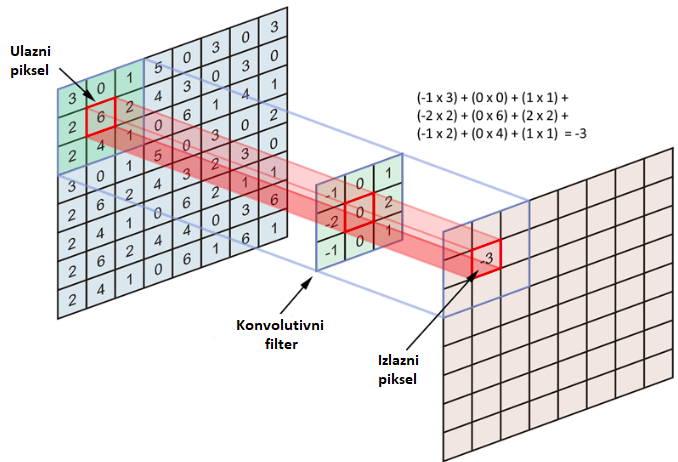
\includegraphics[scale=0.9]{convolution.png}
\caption{Konvolucija primenom filtera dimenzije 3x3 na matricu dimenzije 8x8}
\label{fig:convolution}
\end{figure}

\subsubsection{Prosirivanje}

Formula konvolucije koja je data u poglavlju \ref{konvolucija} nije definisana za sve indekse i=0, m - 1 i j=0, n - 1. Na primer, ako je i, j = 0 i k, l > 0, vrednost fi - k,i - l nije definisana. Ukoliko bi se u obzir uzele samo definisane vrednosti, dimenzija konvolucije bi bila manja od dimenzije matrice f. Medjutim, to nije uvek pozeljno, i moze se izbeci tako sto se vrsi \textbf{prosirivanje} (eng. padding) matrice f, na primer nulama ili vrednostima koje su vec na obodu, tako da velicina rezultujuce matrice bude jednaka velicini matrice f pre prosirivanja. Ovo je prikazano na slici \ref{fig:padding}. Takode, prilikom racunanja konvolucije, filter se duz slike ne mora pomerati za jedan piksel, vec za neki veci \textbf{ korak} (eng. stride).

\begin{figure}[h!]
\begin{center}
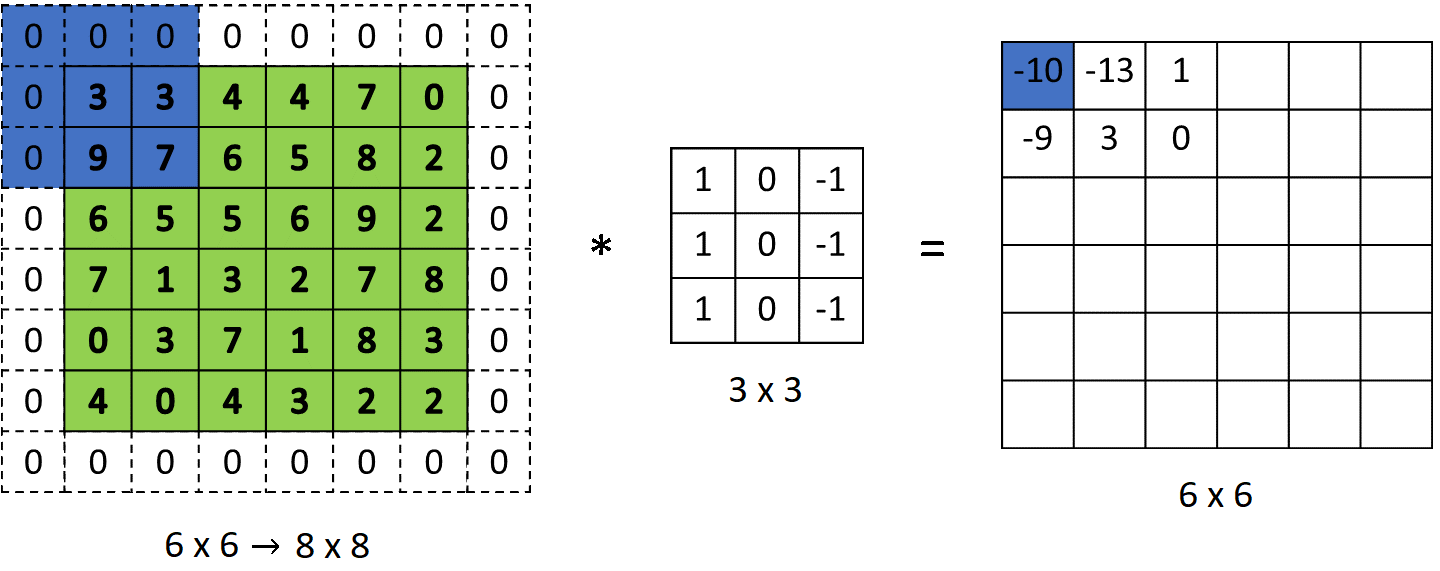
\includegraphics[scale=0.38]{padding.png}
\end{center}
\caption{Primer prosirivanja}
\label{fig:padding}
\end{figure}


\subsubsection{Aktivaciona funkcija}

U konvolutivnim slojevima kao aktivaciona funkcija se najčešće koristi ReLu (Rectified Linear Unit) funkcija. Definisana je kao $$ f(z) = max(0, z). $$ To znači da će negativne piksele mape karakteristika nastale konvolucijom da postavi na nulu i neće aktivirati odgovarajuće neurone. A pozitivne piksele neće menjati. Na taj način, ReLu ne aktivira sve neurone u istom trenutku, čime ubrzava rad mreže i čini je efikasnijom. Na slici \ref{fig:relu_fja} se može videti kako ReLU funkcija izgleda, a na slici \ref{fig:relu_transform} kako se pomoću nje transformiše mapa karakteristika.

\begin{figure}[h!]
\begin{center}
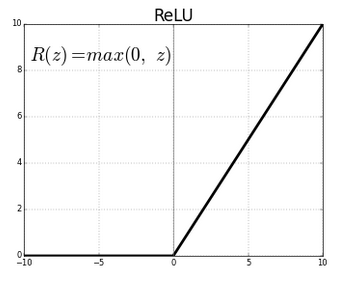
\includegraphics[scale=0.38]{relu2.png}
\end{center}
\caption{Izgled ReLU funkcije}
\label{fig:relu_fja}
\end{figure}


\begin{figure}[h!]
\begin{center}
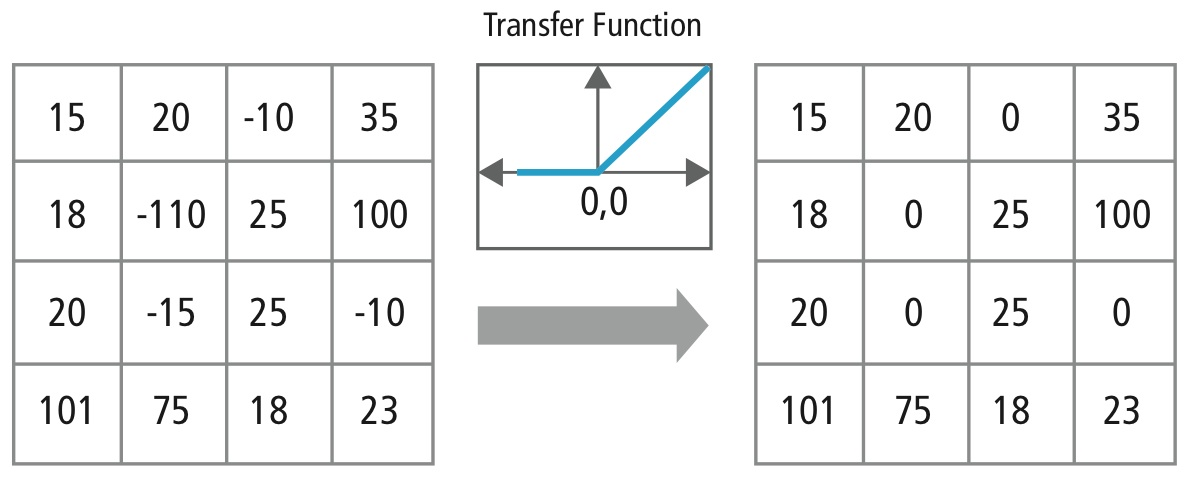
\includegraphics[scale=0.20]{relu1.jpg}
\end{center}
\caption{Primer rada ReLU funkcije nad mapom karakteristika}
\label{fig:relu_transform}
\end{figure}

\newpage

\subsection{Agregacija}

%\footnote{tekst koji se prikazuje kao fusnota}
%\textit{iskosen tekst}
%\ref{sec:primer_koda}

Uloga sloja za agregaciju je smanjenje broja parametara kada su slike prevelike, kao i smanjenje broja racunskih operacija u visim slojevima smanjuje. Agregacija smanjuje dimenzionalnost svake mape, ali zadržava važne informacije. Sve to rezultuje smanjenjem racunske zahtevnosti pri optimizaciji i pomaze u kontroli overfitinga. Zato zelimo da slojevi za agregaciju prate konvolucione slojeve kako bismo postepeno smanjili prostornu veličinu (širinu i visinu) prikaza podataka.

Cesto nas konačni zadatak postavlja neko globalno pitanje o slici, npr., Da li sadrži mačku? Tako da čvorovi našeg zadnjeg sloja moraju biti osetljivi na celi ulaz. Postepenom agregacijom informacija, stvarajuci grublje i grublje mape karakteristika, postize se taj cilj da se na kraju nauci globalna reprezentacija, zadrzavajuci sve prednosti konvolucijskih slojeva na srednjim slojevima obrade.

Sloj agregacije ukrupnjuje informacije, tako sto racuna neku jednostavnu funkciju agregacije susednih jedinica prethodnog sloja, poput maksimuma (eng. Max pooling) [koji vraca maksimalnu vrednost dela slike pokrivene filterom] ili proseka (eng. Average pooling) [koji vraca prosecnu vrednost dela slike pokrivene filterom]. Ukoliko agregira, na primer, 3 x 3 piskela, onda je broj izlaza ovog sloja 9 puta manji od broja izlaza prethodnog. Kada se racuna maksimum, dolazi do zanemarivanje informacije o tome gde je precizno neko svojstvo (poput uspravne linije) pronadeno, ali se ne gubi informacija da je pronadeno. Ovakva vrsta zanemarivanja informacije cesto ne steti cilju koji treba postici. Na primer, ako su na slici pronadeni kljun i krila, informacija o tacnoj pozicjiji najverovatnije nije bitna za odlucivanje da li se na slici nalazi ptica. Ipak, ukoliko je potrebno napraviti mrezu koja igra igru u kojoj su pozicije objekata na ekranu bitne, nije pozeljno koristiti agregaciju.

 Average pooling was often used historically but has recently fallen out of favor compared to the max pooling operation, which has been shown to work better in practice.
 
 Pooling layer downsamples the volume spatially, independently in each depth slice of the input volume.
 
Prva slika (pool): In this example, the input volume of size [224x224x64] is pooled with filter size 2, stride 2 into output volume of size [112x112x64]. Notice that the volume depth is preserved.
 
Druga slika (maxpool): The most common downsampling operation is max, giving rise to max pooling, here shown with a stride of 2. That is, each max is taken over 4 numbers (little 2x2 square).

 
\begin{figure}[h!]
\begin{center}
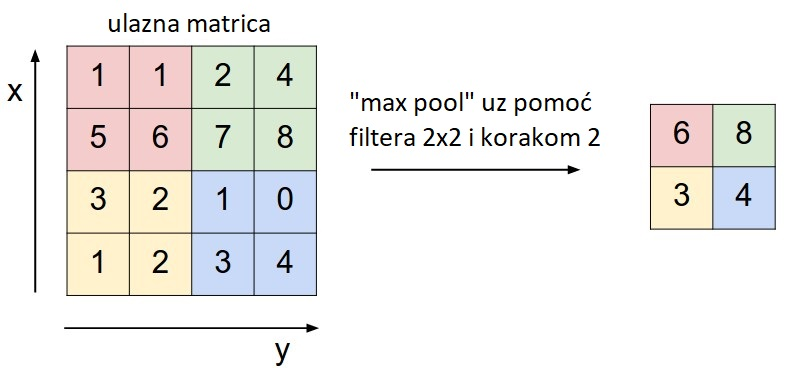
\includegraphics[scale=0.4]{maxpool.jpeg}
\end{center}
\caption{Maxpool}
\label{fig:maxpool}
\end{figure}


\begin{figure}[h!]
\begin{center}
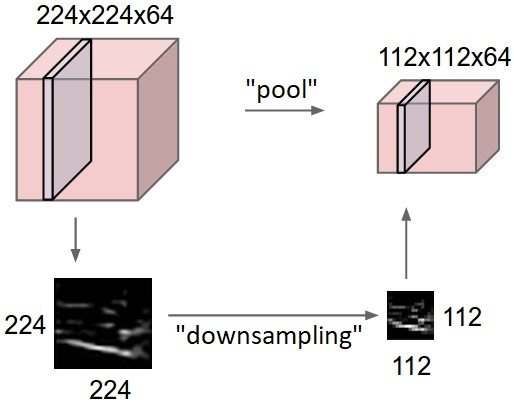
\includegraphics[scale=0.4]{pool.jpeg}
\end{center}
\caption{Pool}
\label{fig:pool}
\end{figure}




\section{Implementacija i eksperimentalni rezultati}
\label{sec:podnaslov8}


Neuronsku mrežu smo implementirale u programskom jeziku Python korišćenjem Keras biblioteke. Kao podatke za trening i testiranje, koristile smo slike iz baze podataka kineskih saobraćajnih znakova \cite{CTSD}. Baza sadrži 6164 slika saobraćajnih znakova podeljenih u 58 klasa, pri čemu trening skup sadrži 4170, a test skup 1994 slike. Međutim, nisu sve klase imale podjednak broj slika. Za neke je postojalo 5 slika na kojima bi mreza mogla da trenira, a za neke oko 400. Takođe, zbog prevelike količine podataka, izvršavanje programa je bilo mnogo sporo. Zbog svega toga, odlučile smo da koristimo samo jedan deo te baze i izdvojile 10 klasa koje su imale približno jednak broj slika. Nakon toga, dobile smo trening skup od 1693 slika i test skup od 764 slike. Na slici \ref{fig:trening_skup} je prikazan po jedan znak iz svake klase trening skupa, zajedno sa brojem elemenata te klase. Slično, ti podaci o test skupu, mogu se videti na slici \ref{fig:test_skup}.

\begin{figure}[h!]
\begin{center}
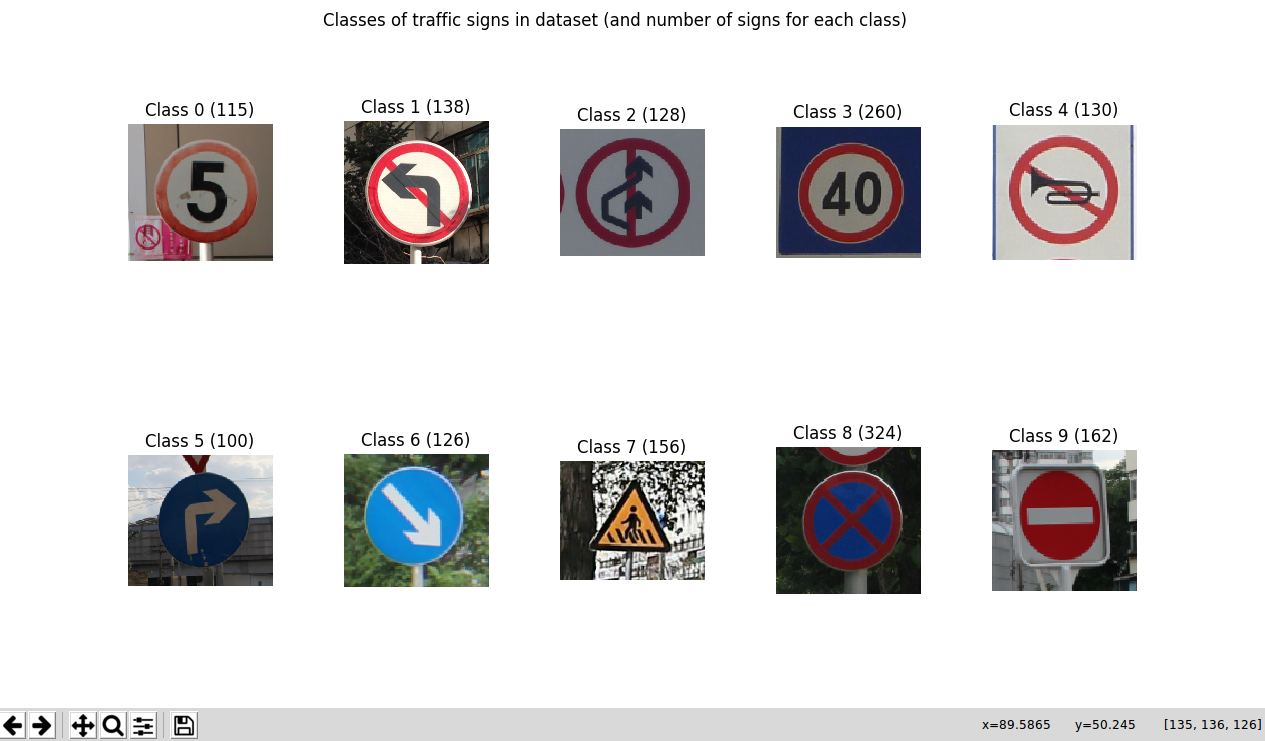
\includegraphics[scale=0.25]{trening_skup.png}
\end{center}
\caption{Trening skup}
\label{fig:trening_skup}
\end{figure}

\begin{figure}[h!]
\begin{center}
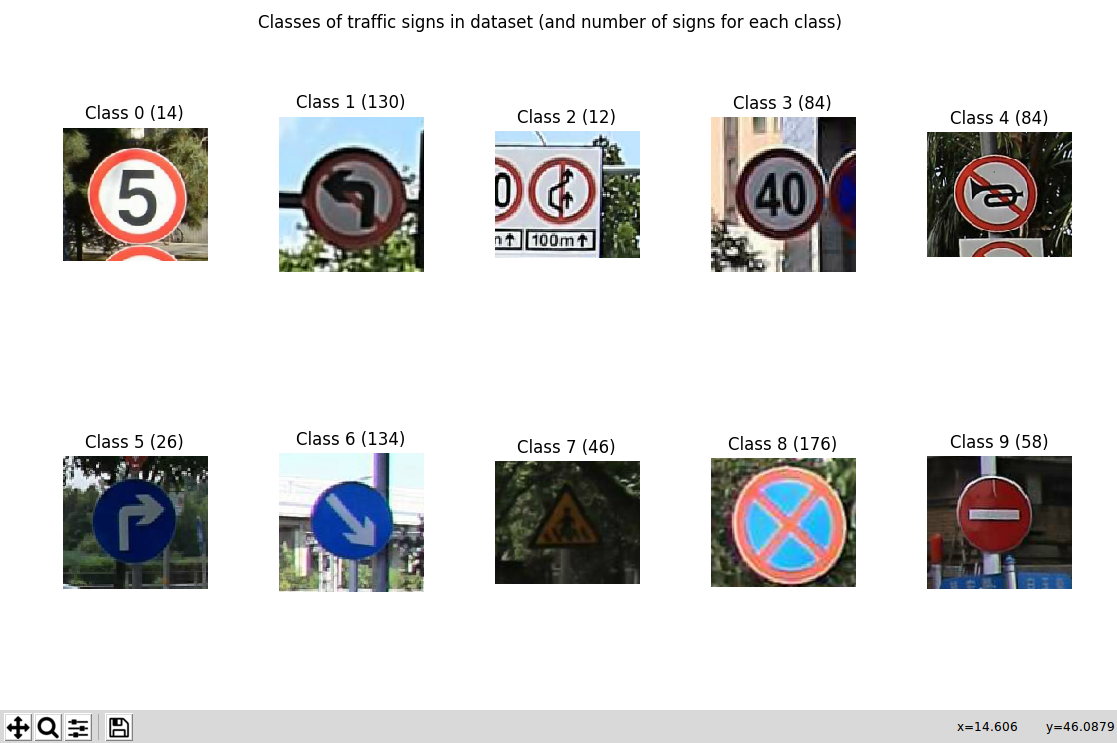
\includegraphics[scale=0.25]{test_skup.png}
\end{center}
\caption{Test skup}
\label{fig:test_skup}
\end{figure}

U narednim poglavljima će biti predstavljeni neki od modela konvolutivnih neuronskih mreža koje smo pravile, a koje su davale najbolje rezultate.

\subsection{Model 1}
\label{sec:model_1}

Jedan od prvih modela koji je imao veći uspeh na test podacima prikazan je u kodu \ref{code:model1}. Sastoji se iz četiri konvolutivna, dva agregirajuća i dva potpuno povezana sloja. Detaljna arhitektura mreže se može videti na slici \ref{fig:model1_arh}. U svim konvolutivnim slojevima veličina jezgra je 3x3, a broj filtera na izlazu iz konvolucije je 32. Takođe, u svakom se koristi ReLU aktivaciona funkcija. U sloju agregacije, sažimanje se vrši biranjem maksimalne vrednosti dela mape karakteristika koji je prekriven filterom. Kako ne bi došlo do preprilagodjavanja modela trening podacima, povremeno je, pomoću funkcije Dropoup(), isključivan određen broj nasumično odabranih neurona. Nakon agregacija je isključeno 20\% neurona, a pre poslednjeg, potpuno povezanog, sloja 50\%. Poslednji potpuno povezani sloj ima onoliko neurona koliko ima klasa i koristi softmax aktivacionu funkciju.

Učenje modela je sprovedeno u 30 epoha. Batch size je postavljen na 32, što znači da će u svakoj iteraciji biti uzeta 32 primerka iz trening skupa koja će biti propagirana kroz mrežu. Optimizacija modela je izvršena pomoću gradijentnog spusta. Takođe, pre početka treninga, sve slike su skalirane na istu veličinu, 64x64 piksela.


\begin{lstlisting}[caption={Model 1},frame=single, label=code:model1]
def cnn_model():
    
    model = Sequential()

    model.add(Conv2D(filters = 32, kernel_size = (3, 3), 
    		padding='same', input_shape=(IMG_SIZE, IMG_SIZE, 3), 
    		data_format="channels_last", activation='relu'))
    model.add(Conv2D(filters = 32, kernel_size = (3, 3), 
    		activation='relu'))
    model.add(MaxPooling2D(pool_size=(2, 2)))
    model.add(Dropout(0.2))

    model.add(Conv2D(filters = 32, kernel_size = (3, 3), 
    		padding='same', activation='relu'))
    model.add(Conv2D(filters = 32, kernel_size = (3, 3), 
    		activation='relu'))
    model.add(MaxPooling2D(pool_size=(2, 2)))
    model.add(Dropout(0.2))
    
    model.add(Flatten())
    model.add(Dense(512, activation='relu'))
    model.add(Dropout(0.5))
    model.add(Dense(NUM_OF_CLASSES, activation='softmax'))
    
    model.summary()
    return model


batch_size = 32
epochs = 30
lr = 0.01   #learning rate

model = cnn_model()

# optimizacija pomocu gradijentnog spusta
sgd = SGD(lr=lr, decay=1e-6, momentum=0.9, nesterov=True)

model.compile(loss='categorical_crossentropy', optimizer=sgd, 
			  metrics=['accuracy'])

def lr_schedule(epoch):
    return lr * (0.1 ** int(epoch / 10))

model.fit(images, classes,
          batch_size=batch_size,
          epochs=epochs,
          validation_split=0.2,
          callbacks=[LearningRateScheduler(lr_schedule), 
          			 ModelCheckpoint('model.h5', save_best_only=True)])
\end{lstlisting}


\begin{figure}[h!]
\begin{center}
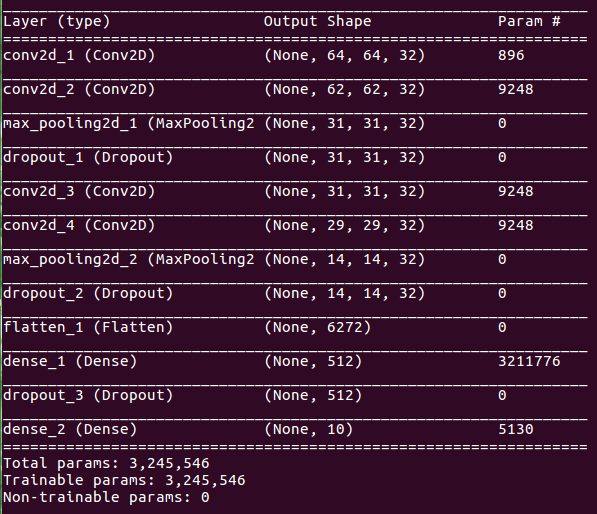
\includegraphics[scale=0.45]{model1_arhitektura.png}
\end{center}
\caption{Slojevi modela neuronske mreže}
\label{fig:model1_arh}
\end{figure}

Na slici \ref{fig:model1_trening_acc} možemo videti da je preciznost modela na trening skupu tokom poslednje tri epohe varirala oko 0.99 i 1.0. Na slici \ref{fig:model1_test_acc} možemo videti kako se model pokazao na test skupu. Preciznost (\textit{accuracy}, tj. broj tačno klasifikovanih instanci / ukupan broj instanci) je jednaka 0.882. Vidimo da je i preciznost (\textit{precision}) koja se odnosi na svaku od klasa dosta visoka (osim za klase 0 i 5)

\begin{figure}[h!]
\begin{center}
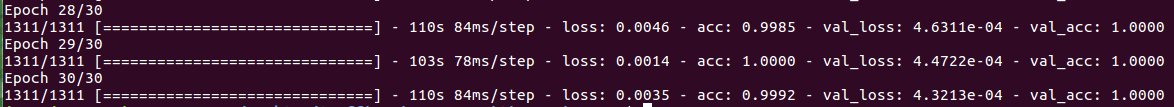
\includegraphics[scale=0.35]{model1_trening_acc.png}
\end{center}
\caption{Preciznost na trening podecima}
\label{fig:model1_trening_acc}
\end{figure}

\begin{figure}[h!]
\begin{center}
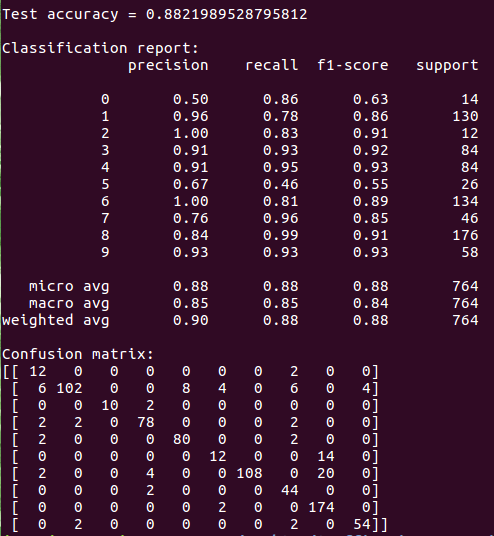
\includegraphics[scale=0.45]{model1_test_acc.png}
\end{center}
\caption{Preciznost na test podecima}
\label{fig:model1_test_acc}
\end{figure}

\newpage

\subsection{Model 2:  LeNet-5}
\label{sec:model_2}


Još bolje rezultate smo dobile pomoću LeNet-5 mreže \cite{leNet}. LeNet-5 mrežu je 1990ih napravio Yann LeCunn. Mreža se sastoji iz 7 slojeva, pri čemu se ne računa ulazni sloj. Sve slike smo skalirale na večičinu 32x32 piksela, jer ova mreža kao ulaz očekuje slike tih dimenzija. Prvi konvolutivni sloj na izlazu daje 6 mapa karakteristika, koristi jezgro veličine 3x3 i kao aktivacionu funkciju koristi ReLU. Nakon njega sledi sloj agregacije u kom se sažimanje vrši biranjem prosečne vrednosti dela mape karakteristika koji je prekriven filterom. 
Još jednom se ponavljaju ova dva sloja, s tim što sada konvolutivni sloj vraća 16 mapa karakteristika. Nakon ispravljanja mape karakteristika u vektor, taj vektor se prosleđuje potpuno povezanom sloju koji se sastoji iz 120 neurona i koristi ReLU aktivacionu funkciju. Nakon toga sledi potpuno povezani sloj od 84 neurona koji, takođe, koristi ReLU aktivacionu funkciju. I, na kraju, ostaje još jedan potpuno povezani sloj koji ima onoliko neurona koliko ima klasa i koji koristi softmax aktivacionu funkciju. U kodu \ref{code:leNet} je data implementacija LeNet-5 mreže, a na slici \ref{fig:leNet_arh} je prikazana njena detaljna arhitektura.

\begin{lstlisting}[caption={LeNet-5},frame=single, label=code:leNet]
def cnn_model():
    
    model = Sequential()

    model.add(Conv2D(filters=6, kernel_size=(3, 3), 
    		activation='relu', input_shape=(IMG_SIZE, IMG_SIZE, 3),
    		data_format="channels_last"))
    model.add(AveragePooling2D())

    model.add(Conv2D(filters=16, kernel_size=(3, 3), 
    		activation='relu'))
    model.add(AveragePooling2D())

    model.add(Flatten())
    model.add(Dense(units=120, activation='relu'))
    model.add(Dense(units=84, activation='relu'))
    model.add(Dense(units=NUM_OF_CLASSES, activation = 'softmax'))
    
    model.summary()
    return model


batch_size = 32   
epochs = 20
lr = 0.01         

model = cnn_model()

model.compile(loss=keras.losses.categorical_crossentropy, 
			  optimizer=keras.optimizers.Adam(),
			  metrics=['accuracy'])

def lr_schedule(epoch):
    return lr * (0.1 ** int(epoch / 10))

model.fit(images, classes,
          batch_size=batch_size,
          epochs=epochs,
          validation_split=0.2,
          callbacks=[LearningRateScheduler(lr_schedule), 
          			 ModelCheckpoint('model.h5', save_best_only=True)])
\end{lstlisting}


\begin{figure}[h!]
\begin{center}
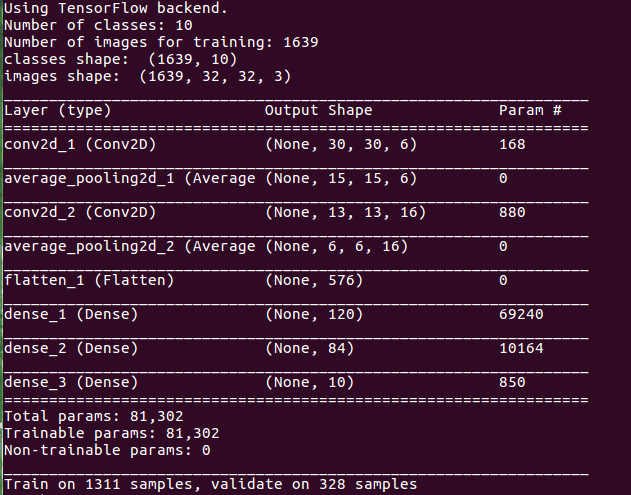
\includegraphics[scale=0.45]{leNet_arhitektura.png}
\end{center}
\caption{Slojevi modela leNet-5 neuronske mreže}
\label{fig:leNet_arh}
\end{figure}

Na slici \ref{fig:leNet_trening_acc} možemo videti da je preciznost na trening skupu u poslednje tri iteracije bila najveća moguća, tj 1.00. Na slici \ref{fig:leNet_test_acc} je prikazan rezultat rada modela na test podacima. Preciznost (\textit{accuracy}) iznosi 0.91. Takođe vidimo da je preciznost (\textit{precision}) za pojedinačne klase visoka. Na osnovu matrice konfuzije može se videti da veoma malo podataka pogrešno klasifikuje.


\begin{figure}[h!]
\begin{center}
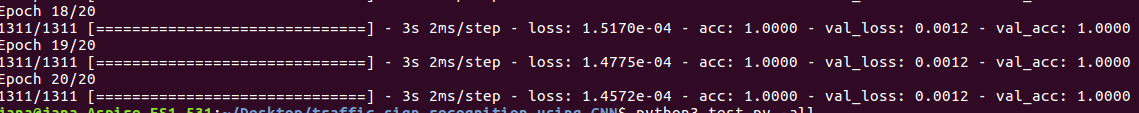
\includegraphics[scale=0.35]{leNet_trening_acc.png}
\end{center}
\caption{Preciznost na trening podecima}
\label{fig:leNet_trening_acc}
\end{figure}

\begin{figure}[h!]
\begin{center}
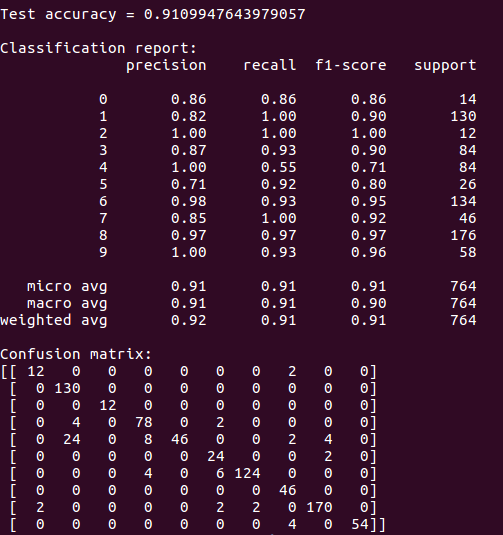
\includegraphics[scale=0.45]{leNet_test_acc.png}
\end{center}
\caption{Preciznost na test podecima}
\label{fig:leNet_test_acc}
\end{figure}




\newpage

\section{Zaključak}
\label{sec:zakljucak}

\newpage

\addcontentsline{toc}{section}{Literatura}
\appendix
\bibliography{seminarski} 
\bibliographystyle{plain}

\newpage

\appendix
\section{Dodatak}
\subsection{Podnaslov 1}
%\label{sec:???}

\textbf{Dodatna objasnjenja} %TODO: Ubaciti u fusnote!


By visualizing the output from different convolution layers in this manner, the most crucial thing that you will notice is that the layers that are deeper in the network visualize more training data specific features, while the earlier layers tend to visualize general patterns like edges, texture, background etc.

This knowledge is very important when you use Transfer Learning whereby you train some part of a pre-trained network (pre-trained on a different dataset, like ImageNet in this case) on a completely different dataset. The general idea is to freeze the weights of earlier layers, because they will anyways learn the general features, and to only train the weights of deeper layers because these are the layers which are actually recognizing your objects.

Convolved Feature, Activation Map or Feature Map is the output volume formed by sliding the filter over the image and computing the dot product.
Perceptrons come first in 1950s, and it uses a brittle activation function to do classification, so if w*x is greater than some value it predicts positive, otherwise negative.

Neurons uses a softer activation function by introducing a sigmoid function, a tanh function or other activation functions to pass on values to other neurons in the network.

So perceptrons do not use in a network setting, they do classification on their own, hence they can’t classify XOR, however neurons can because they all contribute forward to the final output, using more complicated structure(i.e. multiple layers in network), they are able to classify XOR and other complicated problems.

A CNN, in specific, has one or more layers of convolution units. A convolution unit receives its input from multiple units from the previous layer which together create a proximity. Therefore, the input units (that form a small neighborhood) share their weights.

The convolution units (as well as pooling units) are especially beneficial as:

They reduce the number of units in the network (since they are many-to-one mappings). This means, there are fewer parameters to learn which reduces the chance of overfitting as the model would be less complex than a fully connected network.
They consider the context/shared information in the small neighborhoods. This future is very important in many applications such as image, video, text, and speech processing/mining as the neighboring inputs (eg pixels, frames, words, etc) usually carry related information.


\end{document}
